\documentclass[t]{beamer}

\usepackage[utf8]{inputenc}
\usepackage[T1]{fontenc}
\usepackage{lmodern}
\usepackage{exscale} % Fixes issues with lmodern math symbols

\usepackage{tikz}
\usetikzlibrary{positioning, arrows.meta}

\tikzset{%
  eda/.style={-{Latex[scale=3]}},
  edc/.style={eda, color=black!25},
  rv/.style={draw, circle, minimum size=3cm},
  ob/.style={rv, fill=black!25}
}

\usepackage{listings}
\lstset{%
  language=Lisp,
  basicstyle=\ttfamily\footnotesize
}

\usepackage[orientation=portrait,size=a0,scale=1.4]{kthposter}

\title{%
  Combining Static and Dynamic Optimizations Using Closed-Form Solutions
}
\author{%
  Daniel Lundén\inst{1}
  \and
  David Broman\inst{1}
  \and
  Lawrence M. Murray\inst{2}
}
\institute{%
  \inst{1}KTH Royal Institute of Technology, Sweden
  \qquad
  \inst{2}Uppsala University, Sweden
}

\logoLeft{%
  
\includegraphics[height=7cm, width=7cm]{img/logo} \\
  
\includegraphics[height=7cm, width=7cm]{img/ulogo}
}

\logoRight{%
  \hfill
  \begin{tikzpicture}
    \node[inner sep=0cm] (pic)%
      {
\includegraphics[height=7cm, width=7cm, keepaspectratio]{img/ssf}};
    \node[below = of pic, xshift=-3mm, align=center]
      {Financially supported \\[1ex] by the Swedish Foundation \\[1ex] for
      Strategic Research.};
  \end{tikzpicture}
}

\footline{%
  This project is financially supported by the Swedish Foundation for
  Strategic Research (ASSEMBLE RIT15-0012).
}

\newlength{\cheight}
\setlength{\cheight}{93cm}

\begin{document}
\begin{frame}[fragile]{}
  \begin{minipage}[c][\cheight][t]{0.48\linewidth}
    \begin{block}{Introduction}
      \begin{itemize}
        \item
          \textbf{Probabilistic programming languages} increases
          \emph{expressiveness} compared to probabilistic graphical models
          through:
          \begin{itemize}
            \normalsize
            \item Stochastic branching
            \item Recursion
          \end{itemize}

        \item
          \vspace{1cm}
          \textbf{Importance sampling} methods (including \textbf{sequential
          Monte Carlo methods}) perform inference in probabilistic programming
          languages through \emph{repeated execution} of programs.

        \item
          \vspace{1cm}
          \textbf{Static optimizations} are program transformations performed
          prior to execution.

          \textbf{\textcolor{blue}{Benefit}}: we can optimize programs offline
          with minimal overhead during execution.

        \item
          \vspace{1cm}
          \textbf{Dynamic optimizations} are optimizations performed during
          execution.

          \textbf{\textcolor{blue}{Benefit}}: we have access to information
          only available during execution.

        \item
          \vspace{1cm}
          The local \textbf{closed-form solutions} we use here are:

          Given
          $p(x)$,
          $p(y|x)$ and
          $y$,
          \textcolor{blue}{$p(y)$} and \textcolor{blue}{$p(x|y)$} can be
          calculated
          in closed-form.
      \end{itemize}
    \end{block}

    \vfill

    \begin{block}{Objective of optimization}
      \begin{itemize}
        \item \textbf{Maximizing quality of inference} (e.g.\ low variance of
          estimators).

        \item
          \vspace{1cm}
          \textbf{Minimizing execution time of inference}.
    \end{itemize}
  \end{block}

  \vfill

  \begin{block}{The need for static optimization}
    \textbf{A probabilistic program (Anglican)}

    \vspace{5mm}
    \begin{center}
      \begin{tabular}{c}
        \begin{lstlisting}
(defquery static
  (let [data [0.4 0.9 -0.1 -1.3 0.2 2.1]
        x (sample (normal 0 1))]
    (observe (normal x 1) (first data))
    (loop [x x, data (rest data)]
      (if (seq data)
        (let [x (sample (normal x 1))]
          (observe (if (> (count data) 1)
                     (normal x 1) (normal 0 (+ 1 (abs x))))
                   (first data))
          (recur x (rest data))) x))))
        \end{lstlisting}
      \end{tabular}
    \end{center}
    \vspace{10mm}

    \textbf{Corresponding graphical model}

    \vspace{5mm}
    \begin{center}
      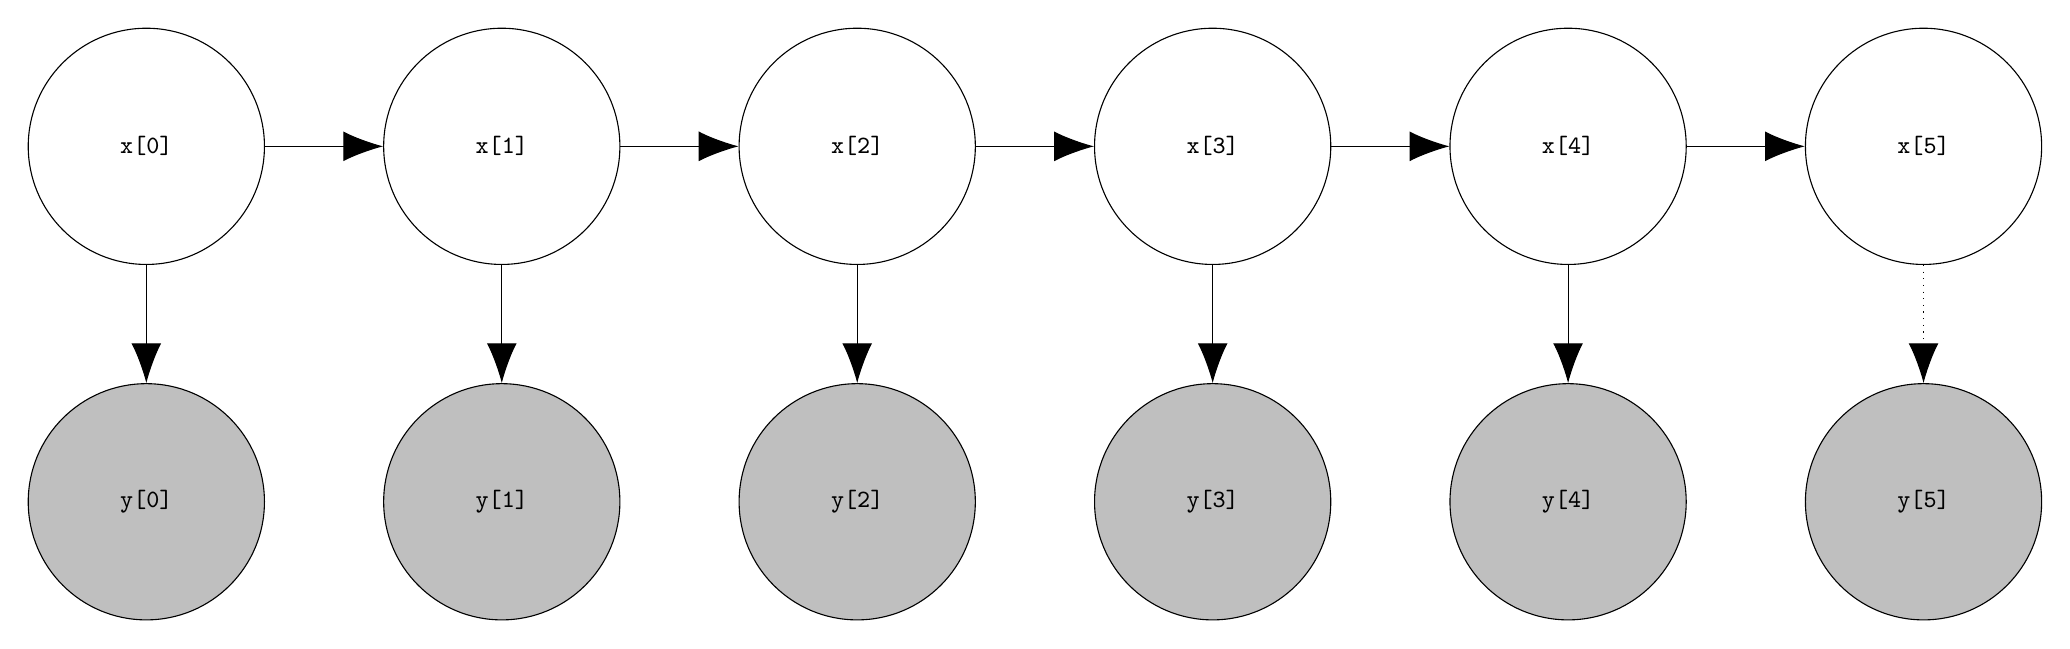
\begin{tikzpicture}
        \node[rv] (x0) []                   {\small \texttt{x[0]}};
        \node[rv] (x1) [right = 15mm of x0] {\small \texttt{x[1]}};
        \node[rv] (x2) [right = 15mm of x1] {\small \texttt{x[2]}};
        \node[rv] (x3) [right = 15mm of x2] {\small \texttt{x[3]}};
        \node[rv] (x4) [right = 15mm of x3] {\small \texttt{x[4]}};
        \node[rv] (x5) [right = 15mm of x4] {\small \texttt{x[5]}};
        \node[ob] (y0) [below = 15mm of x0] {\small \texttt{y[0]}};
        \node[ob] (y1) [below = 15mm of x1] {\small \texttt{y[1]}};
        \node[ob] (y2) [below = 15mm of x2] {\small \texttt{y[2]}};
        \node[ob] (y3) [below = 15mm of x3] {\small \texttt{y[3]}};
        \node[ob] (y4) [below = 15mm of x4] {\small \texttt{y[4]}};
        \node[ob] (y5) [below = 15mm of x5] {\small \texttt{y[5]}};
        \path[eda]
        (x0) edge (x1)
        (x1) edge (x2)
        (x2) edge (x3)
        (x3) edge (x4)
        (x4) edge (x5)
        (x0) edge (y0)
        (x1) edge (y1)
        (x2) edge (y2)
        (x3) edge (y3)
        (x4) edge (y4)
        (x5) edge[dotted] (y5);
      \end{tikzpicture}
    \end{center}
    \vspace{10mm}

    \textbf{Optimized program (partially solved analytically)}

    \vspace{5mm}

    \begin{center}
      \begin{tabular}{c}
        \begin{lstlisting}
(defquery static-opt
  (let [data [2.1]
        x (sample (normal -0.157 (sqrt 1.617)))]
    (observe (normal 0 (+ 1 (abs x))) (first data)) x))
        \end{lstlisting}
      \end{tabular}
    \end{center}
    \vspace{10mm}

    \textbf{Conclusion}
    \begin{itemize}
      \item When our program $\equiv$ a graphical model, we should always do
        these types of optimizations statically.
    \end{itemize}
  \end{block}
\end{minipage}
\hfill
\begin{minipage}[c][\cheight][t]{0.48\linewidth}
  \begin{block}{The need for dynamic optimization}
    \textbf{A probabilistic program (Anglican)}

    \vspace{5mm}
    \begin{center}
      \begin{tabular}{c}
        \begin{lstlisting}
(defquery dynamic
  (let [data [0 -1.1 2.4 1.2 -0.1 -1.4 -1.9]
        x (sample (normal 0 1))
        mix (fn [anc]
              (if (sample (flip 0.5))
                (normal anc 1)
                (normal 0 (+ 1 (abs anc)))))
        foo (fn foo [root depth]
              (let [left (mix root)
                    right (mix root)]
                (if (= depth 1)
                  [left right]
                  (concat (foo (sample left)
                               (- depth 1))
                          (foo (sample right)
                               (- depth 1))))))
        leaves (foo x 3)]
    (map (fn [dist obs] (observe dist obs))
         leaves data) x))
        \end{lstlisting}
      \end{tabular}
    \end{center}
    \vspace{10mm}

    \textbf{Corresponding graphical model}

    \vspace{5mm}
    \begin{center}
      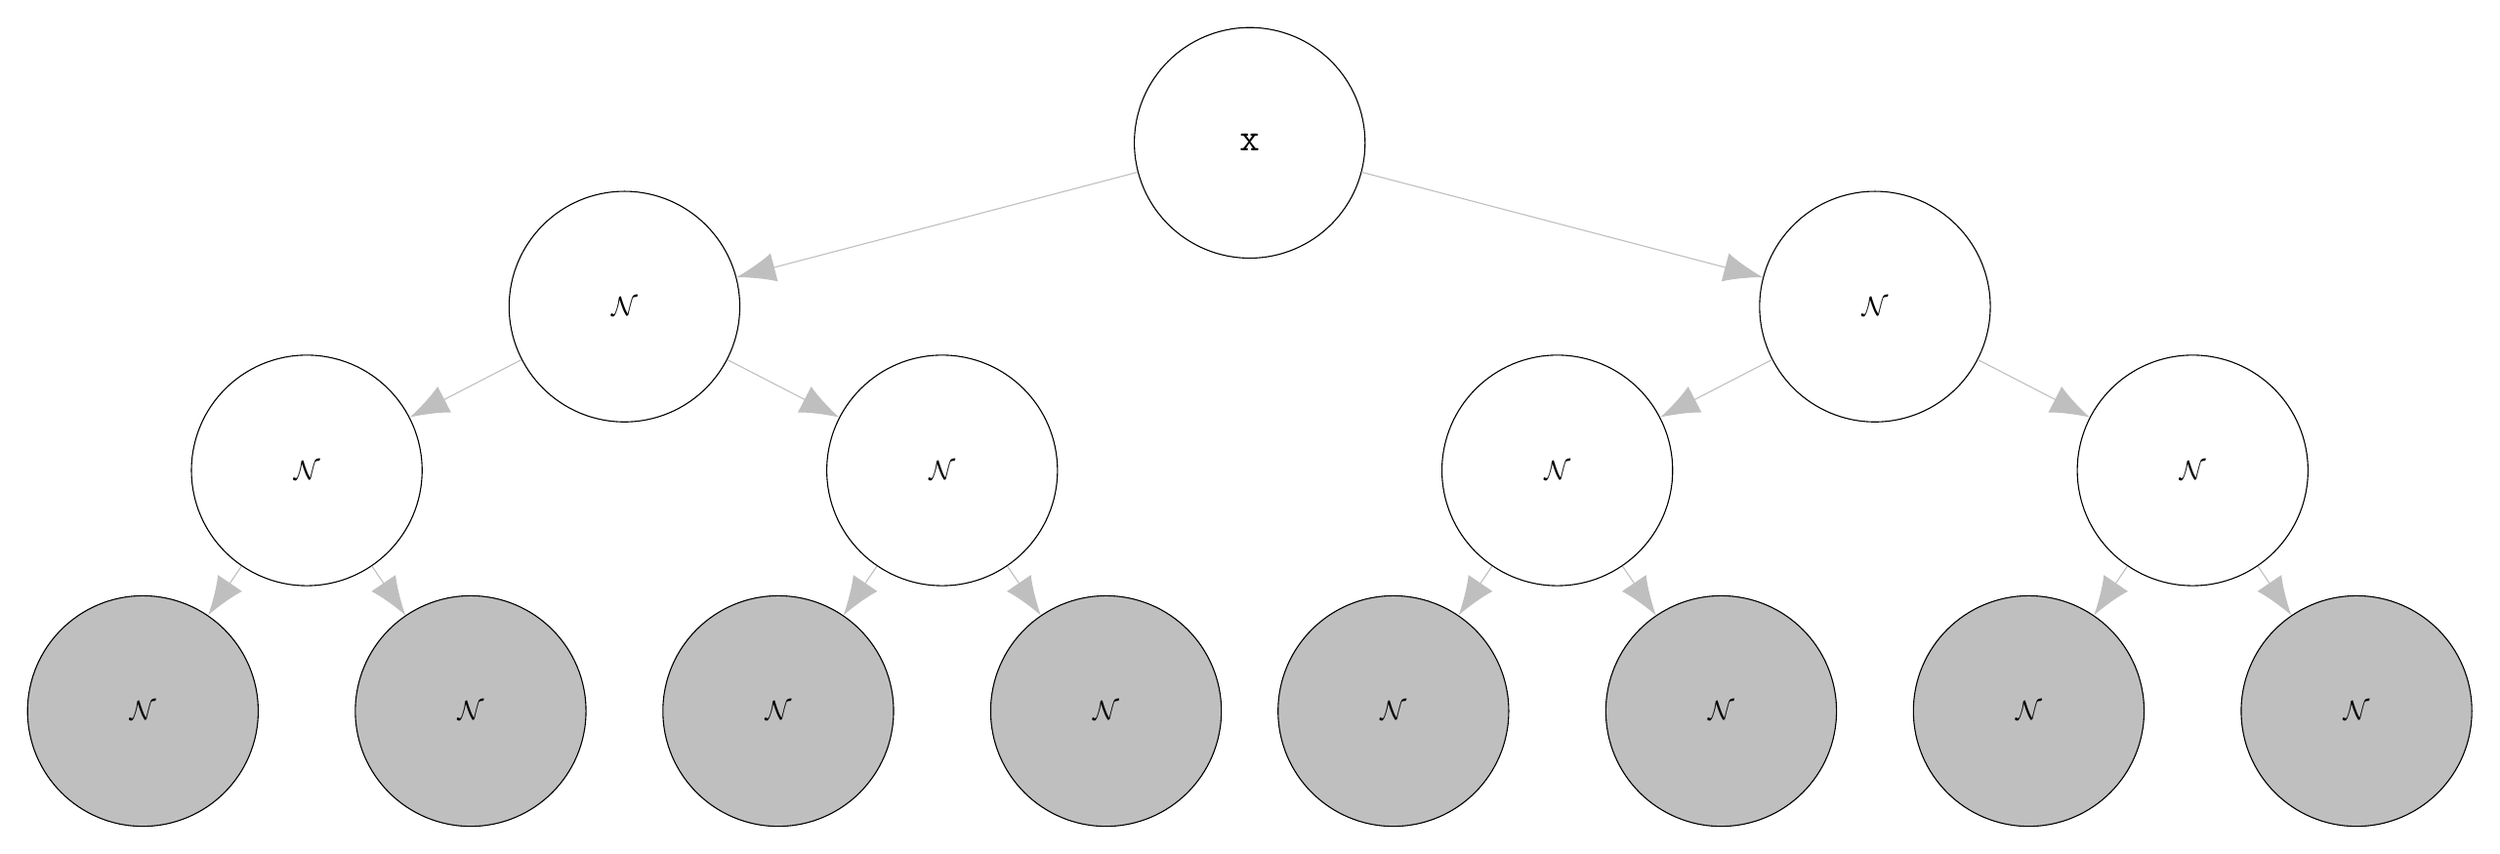
\begin{tikzpicture}
        \node[rv] (1)  []                                 {\Large \texttt{x}};
        \node[rv] (2)  [below left  = 0mm and 60mm  of 1] {$\mathcal{N}$};
        \node[rv] (3)  [below right = 0mm and 60mm  of 1] {$\mathcal{N}$};
        \node[rv] (4)  [below left  = 0mm and 20mm of 2]  {$\mathcal{N}$};
        \node[rv] (5)  [below right = 0mm and 20mm of 2]  {$\mathcal{N}$};
        \node[rv] (6)  [below left  = 0mm and 20mm of 3]  {$\mathcal{N}$};
        \node[rv] (7)  [below right = 0mm and 20mm of 3]  {$\mathcal{N}$};
        \node[ob] (8)  [below left =  10mm and 0mm of 4]    {$\mathcal{N}$};
        \node[ob] (9)  [below right = 10mm and 0mm of 4]   {$\mathcal{N}$};
        \node[ob] (10) [below left =  10mm and 0mm of 5]    {$\mathcal{N}$};
        \node[ob] (11) [below right = 10mm and 0mm of 5]   {$\mathcal{N}$};
        \node[ob] (12) [below left =  10mm and 0mm of 6]    {$\mathcal{N}$};
        \node[ob] (13) [below right = 10mm and 0mm of 6]   {$\mathcal{N}$};
        \node[ob] (14) [below left =  10mm and 0mm of 7]    {$\mathcal{N}$};
        \node[ob] (15) [below right = 10mm and 0mm of 7]   {$\mathcal{N}$};
        \path[edc]
        (1) edge (2)
        (1) edge (3)
        (2) edge (4)
        (2) edge (5)
        (3) edge (6)
        (3) edge (7)
        (4) edge (8)
        (4) edge (9)
        (5) edge (10)
        (5) edge (11)
        (6) edge (12)
        (6) edge (13)
        (7) edge (14)
        (7) edge (15);
      \end{tikzpicture}
    \end{center}
    \vspace{10mm}

    \textbf{Conclusion}
    \begin{itemize}
      \item Static optimization not a good idea due to stochastic branching
        \vspace{5mm}
      \item \textbf{Delayed sampling} is a dynamic approach for these
        situations (see references below)
    \end{itemize}
  \end{block}
  \vfill

  \begin{block}{Challenges}
    \begin{itemize}
      \item When do we use which approach?

      \item
        \vspace{1cm}
        Can we get the best of both worlds by \textbf{combining} the two
        approaches \textbf{within} a single program?

      \item
        \vspace{1cm}
        Can we define and find \textbf{optimal} combinations?
    \end{itemize}

    \vspace{1cm}
    \begin{center}
      
\includegraphics[width=0.17\textwidth]{img/challenges}
    \end{center}
  \end{block}

  \vfill

  \begin{block}{References}
    \begin{itemize}
      \item
        Lawrence M. Murray, Daniel Lundén, Jan Kudlicka, David Broman, and
        Thomas B. Schön. 2017. \emph{Delayed Sampling and Automatic
        Rao--Blackwellization of Probabilistic Programs}. To appear in
        proceedings of AISTATS 2018.

      \item
        \vspace{1cm}
        Daniel Lundén. 2017. \emph{Delayed sampling in the
        probabilistic programming language Anglican}. Master's thesis. KTH
        Royal Institute of Technology.
    \end{itemize}
  \end{block}

\end{minipage}
\end{frame}
\end{document}
